\section{实验与分析}

\subsection{数据集与实验设置}
合成低照度实验使用 20 张 Kodak clean 图像作为参考图像，按照
\begin{equation}
I_{low}=(\alpha I)^{\gamma}+n
\end{equation}
构造低照度样本。基础退化条件为 $\alpha=0.3,\gamma=2.0,\sigma=0.02$，更强退化条件为 $\alpha=0.2,\gamma=2.2,\sigma=0.03$。真实低照度实验使用 6 张自行拍摄图像，仅用于主观可视化与无参考评价。

对比方法包括：低照度输入、HE、固定 CLAHE、去噪后 CLAHE 和本文方法。合成数据定量评价采用 PSNR、SSIM、NAR 和 Mean~Y；真实低照度图像采用 LOE\cite{wang2013loe} 以及基于 clean 图像自然场景统计拟合的 NIQE-like 自然度分数，其设计思想参考了 NIQE 指标\cite{mittal2012niqe}。LOE 越低表示光照顺序破坏越小；NIQE-like 分数越低表示图像统计特性越接近 clean 参考图像。

\subsection{主实验结果}
主实验结果如表~\ref{tab:main} 所示。固定 CLAHE 在基础退化条件下取得了最高的 SSIM（0.168880）和较低的 NAR（7.244474），去噪后 CLAHE 则取得了最低的 NAR（3.368907），说明这两种 baseline 在结构稳定性和噪声控制方面整体更稳。相比之下，本文方法的 PSNR 为 8.332612、SSIM 为 0.140888、NAR 为 11.482148、Mean~Y 为 18.209705，表现为一种更偏保守的亮度增强与噪声控制折中，而非最终画质最优。

\begin{table}[H]
\centering
\caption{基础退化条件下主实验结果}
\label{tab:main}
\begin{tabular}{lcccc}
\toprule
方法 & PSNR$\uparrow$ & SSIM$\uparrow$ & NAR$\downarrow$ & Mean~Y$\uparrow$ \\
\midrule
Low-light input & 7.231946 & 0.057615 & 1.000000 & 6.417508 \\
HE & 11.806686 & 0.150861 & 348.996833 & 128.706340 \\
CLAHE & 8.408286 & 0.168880 & 7.244474 & 20.142387 \\
Denoise+CLAHE & 8.104546 & 0.159518 & 3.368907 & 16.591029 \\
Proposed & 8.332612 & 0.140888 & 11.482148 & 18.209705 \\
\bottomrule
\end{tabular}
\end{table}

图~\ref{fig:real-main} 与图~\ref{fig:real-main-2} 展示了两组真实低照度图像的对比结果。为避免单独挑选最有利样本，本文仅保留 6 张真实图中本文方法分块相对不明显的两例，并对整条对比图统一进行显示增强，以便观察不同方法的视觉取舍。可以看到，HE 虽然显著提升了整体亮度，但更容易造成过曝和局部不自然；固定 CLAHE 与去噪后 CLAHE 在边缘和自然度上整体更稳；本文方法在这两例中没有出现最严重的过曝，但仍存在偏灰与局部不均匀现象。因此，真实图部分主要用于说明不同方法的取舍，而不作为“本文方法优于 baseline”的证据。

\begin{figure}[H]
\centering
\includegraphics[width=0.95\linewidth]{../figures/real_case_bookshelf_comparison_display.png}
\caption{真实低照度图像方法对比（书架场景，展示版）。顺序为 Input、HE、CLAHE、Denoise+CLAHE、Proposed。整条对比图采用统一显示增强，仅用于提升可读性，不影响定量结果。}
\label{fig:real-main}
\end{figure}

\begin{figure}[H]
\centering
\includegraphics[width=0.95\linewidth]{../figures/real_case_storage_comparison_display.png}
\caption{真实低照度图像方法对比（储物架场景，展示版）。整条对比图采用统一显示增强，仅用于提升可读性，不影响定量结果。}
\label{fig:real-main-2}
\end{figure}

\subsection{局部放大与 clip map 可视化}
为了更直观地展示暗区表现，本文进一步给出局部放大图。图~\ref{fig:crop} 中局部区域由论文专用裁剪流程统一导出，并采用一致的横向比例与显示尺寸；为提升暗区纹理与边缘的可见性，正文中展示的是统一亮度拉伸后的展示版局部图，仅用于可视化分析，不参与定量评价。图~\ref{fig:clipmap} 给出了合成图与真实图上的 clip map，可见高结构区域通常对应更高的 clip limit，而平坦暗区对应较低的增强强度。

\begin{figure}[H]
\centering
\begin{subfigure}[b]{0.48\linewidth}
  \centering
  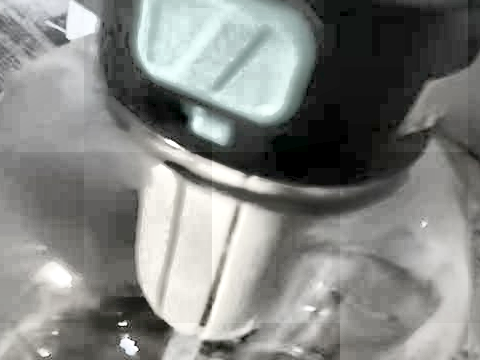
\includegraphics[height=4.8cm]{../figures/fig4_real_crop_display.png}
  \caption{真实图局部放大}
\end{subfigure}
\hfill
\begin{subfigure}[b]{0.48\linewidth}
  \centering
  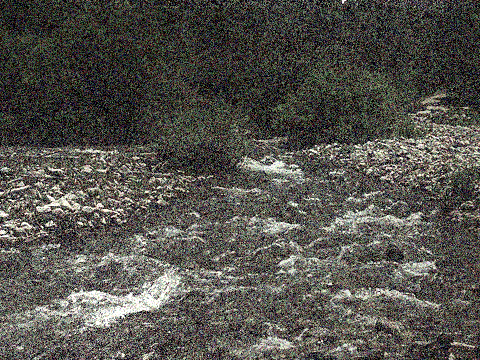
\includegraphics[height=4.8cm]{../figures/fig4_synth_crop_display.png}
  \caption{合成图局部放大}
\end{subfigure}
\caption{真实图与合成图的局部放大展示版。为提升暗区细节的可见性，图中局部区域采用统一亮度拉伸，仅用于可视化分析，不影响定量结果。}
\label{fig:crop}
\end{figure}

\begin{figure}[H]
\centering
\begin{subfigure}[b]{0.48\linewidth}
  \centering
  
\includegraphics[width=\linewidth]{../figures/kodim01_clip_map.png}
  \caption{合成图 clip map}
\end{subfigure}
\hfill
\begin{subfigure}[b]{0.48\linewidth}
  \centering
  
\includegraphics[width=\linewidth]{../figures/real_book_clip_map.png}
  \caption{真实图 clip map}
\end{subfigure}
\caption{自适应 clip map 可视化。}
\label{fig:clipmap}
\end{figure}

\subsection{消融实验}
消融实验结果如表~\ref{tab:ablation} 所示。直接使用原始方差自适应时，SSIM 提升到 0.180278，但 NAR 同时上升到 10.911286，说明更强的自适应增强也会带来更明显的暗区波动放大。继续加入结构方差平滑、噪声抑制和融合策略后，NAR 有下降趋势，但 SSIM 也随之下降，说明本文方法当前更偏向于“抑制极端块效应和增强过强”，而不是单纯追求结构指标最大化。

\begin{table}[H]
\centering
\caption{消融实验结果}
\label{tab:ablation}
\begin{tabular}{lccc}
\toprule
方法 & SSIM$\uparrow$ & NAR$\downarrow$ & Mean~Y$\uparrow$ \\
\midrule
Fixed CLAHE & 0.168880 & 7.244474 & 20.142387 \\
Raw variance adaptive & 0.180278 & 10.911286 & 22.834786 \\
Smoothed variance adaptive & 0.151050 & 17.698392 & 20.579855 \\
Noise-suppressed adaptive & 0.142081 & 16.183597 & 19.048834 \\
Full method & 0.140888 & 11.482148 & 18.209705 \\
\bottomrule
\end{tabular}
\end{table}

\begin{figure}[H]
\centering
\begin{subfigure}[b]{0.95\linewidth}
  \centering
  \includegraphics[width=\linewidth]{../figures/kodim13_ablation_strip.png}
  \caption{原始消融实验输出}
\end{subfigure}

\vspace{0.5em}

\begin{subfigure}[b]{0.95\linewidth}
  \centering
  \includegraphics[width=\linewidth]{../figures/kodim13_ablation_strip_display.png}
  \caption{统一亮度拉伸后的展示版}
\end{subfigure}
\caption{消融实验可视化结果。上：原始消融实验输出；下：对整图统一亮度拉伸后的展示版，仅用于增强印刷可读性，不影响表中定量结果。顺序为 Fixed CLAHE、Raw variance adaptive、Smoothed variance adaptive、Noise-suppressed adaptive、Full method。}
\label{fig:ablation}
\end{figure}

\subsection{融合策略对照}
为验证 tile 间融合对块效应的影响，本文进一步比较了硬拼接、仅 clip map 平滑和双线性融合三种策略，结果如表~\ref{tab:fusion} 所示。硬拼接在 PSNR 上略高，但 NAR 高达 16.183597；加入 clip map 平滑后，NAR 降至 11.794762；双线性融合进一步将 NAR 降至 11.482148，同时主观上块边界过渡最平滑。因此，虽然双线性融合没有在所有定量指标上最优，但它能够最有效地抑制明显块伪影。

\begin{table}[H]
\centering
\caption{融合策略对照结果}
\label{tab:fusion}
\begin{tabular}{lcccc}
\toprule
方法 & PSNR$\uparrow$ & SSIM$\uparrow$ & NAR$\downarrow$ & Mean~Y$\uparrow$ \\
\midrule
Hard stitching & 8.428778 & 0.142081 & 16.183597 & 19.048834 \\
Clipmap smoothing only & 8.357765 & 0.143001 & 11.794762 & 18.486040 \\
Bilinear blending & 8.332612 & 0.140888 & 11.482148 & 18.209705 \\
\bottomrule
\end{tabular}
\end{table}

\begin{figure}[H]
\centering
\begin{subfigure}[b]{0.95\linewidth}
  \centering
  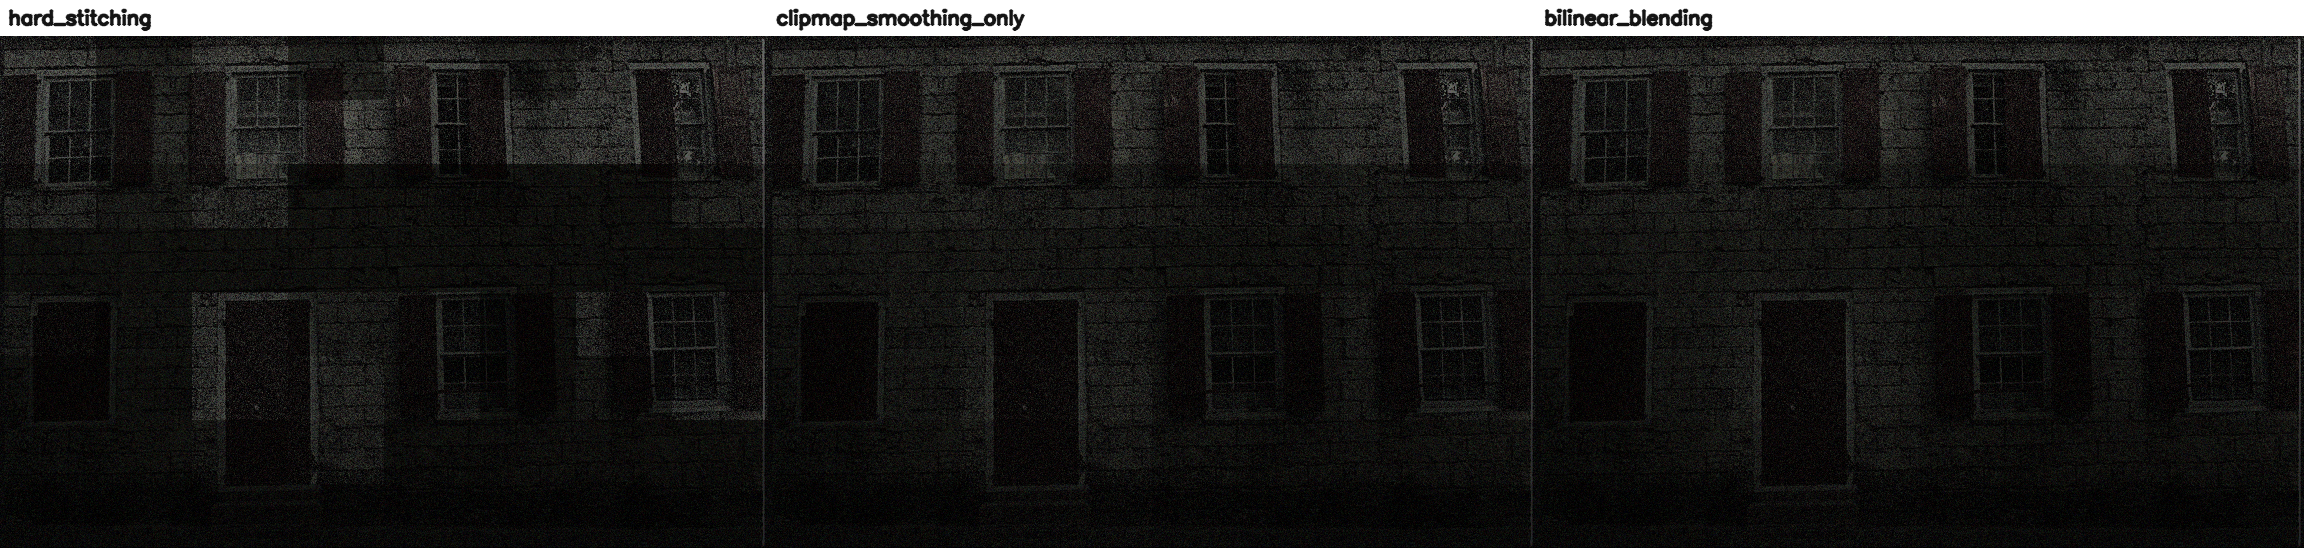
\includegraphics[width=\linewidth]{../figures/kodim01_fusion_strip.png}
  \caption{原始融合策略输出}
\end{subfigure}

\vspace{0.5em}

\begin{subfigure}[b]{0.95\linewidth}
  \centering
  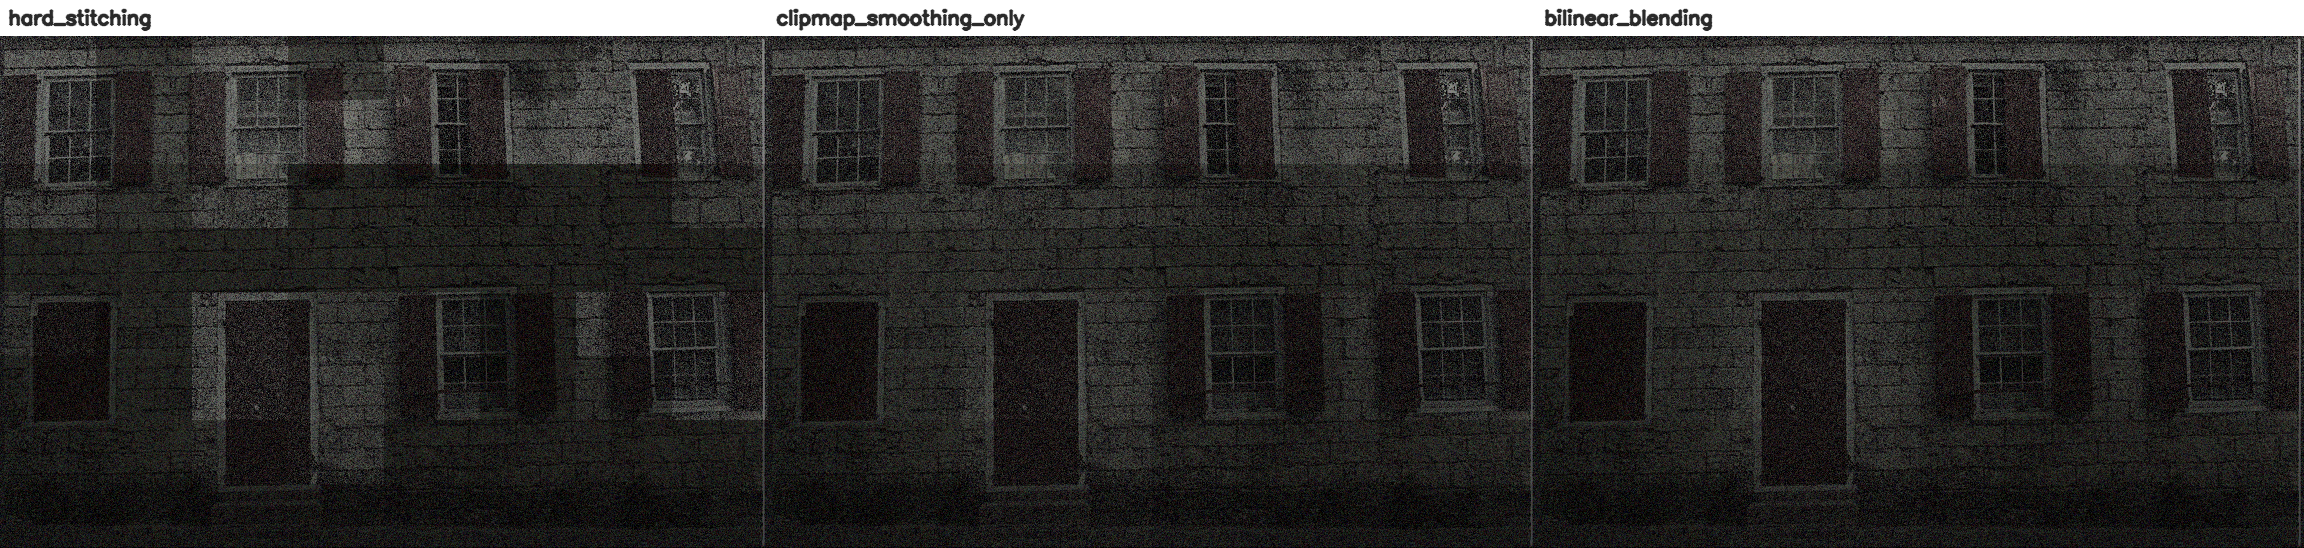
\includegraphics[width=\linewidth]{../figures/kodim01_fusion_strip_display.png}
  \caption{统一亮度拉伸后的展示版}
\end{subfigure}
\caption{融合策略对照图。上：原始融合策略输出；下：统一亮度拉伸后的展示版。可见硬拼接存在明显块边界，而双线性融合在视觉上减弱了块状伪影。顺序为 Hard stitching、Clipmap smoothing only、Bilinear blending。}
\label{fig:fusion}
\end{figure}

\subsection{参数敏感性实验}
参数敏感性结果表明，随着 $\beta$ 从 0.5 增大到 4.0，SSIM 从 0.133338 上升到 0.152642，但 NAR 也从 9.913905 增加到 14.180790；随着 $C_{\max}$ 从 4 增大到 16，SSIM 从 0.133441 提升到 0.181368，但 NAR 也显著上升到 54.076550。这说明增强强度越大，结构恢复指标越高，但噪声与过增强风险也会同步累积，因此本文默认参数更倾向于选择中等增强强度。

\subsection{真实图无参考评价与强退化鲁棒性}
真实低照度图像的无参考评价如表~\ref{tab:real-nr} 所示。本文方法的 Mean~Y 为 90.198739，高于输入图像的 68.684817，说明整体亮度得到提升；其 LOE 为 0.116352，说明在提升亮度的同时也引入了更多光照顺序变化；NIQE-like 分数为 9.581942，优于输入图像但弱于 CLAHE 和 Denoise+CLAHE。结合主观结果可见，本文方法在真实图上更适合被理解为一种增强幅度较温和、但自然度仍有限的折中方案。

\begin{table}[H]
\centering
\caption{真实低照度图无参考评价}
\label{tab:real-nr}
\begin{tabular}{lccc}
\toprule
方法 & LOE$\downarrow$ & NIQE-like$\downarrow$ & Mean~Y$\uparrow$ \\
\midrule
Input & 0.000000 & 10.925067 & 68.684817 \\
HE & 0.016519 & 10.893759 & 128.882222 \\
CLAHE & 0.091568 & 9.049189 & 88.038053 \\
Denoise+CLAHE & 0.091901 & 7.887092 & 88.031926 \\
Proposed & 0.116352 & 9.581942 & 90.198739 \\
\bottomrule
\end{tabular}
\end{table}

在更强退化条件下，主实验结果如表~\ref{tab:hard} 所示。此时所有方法的 PSNR 和 SSIM 均进一步下降，说明任务难度明显增大。去噪后 CLAHE 的 NAR 最低，仅为 1.011724，而本文方法的 NAR 为 4.002738，低于 CLAHE 的 7.918460 和 HE 的 537.711587。这说明在更强退化场景下，本文方法虽然结构指标较弱，但相较固定 CLAHE 的噪声放大更温和。

\begin{table}[H]
\centering
\caption{更强退化条件下主实验结果}
\label{tab:hard}
\begin{tabular}{lcccc}
\toprule
方法 & PSNR$\uparrow$ & SSIM$\uparrow$ & NAR$\downarrow$ & Mean~Y$\uparrow$ \\
\midrule
Low-light input & 6.991349 & 0.042855 & 1.000000 & 4.027395 \\
HE & 9.192554 & 0.038398 & 537.711587 & 120.477110 \\
CLAHE & 7.737174 & 0.098107 & 7.918460 & 14.417101 \\
Denoise+CLAHE & 7.557162 & 0.119254 & 1.011724 & 11.758983 \\
Proposed & 7.287493 & 0.069496 & 4.002738 & 8.100744 \\
\bottomrule
\end{tabular}
\end{table}

\subsection{讨论}
综合以上实验可以看出，本文方法目前并未在所有指标上优于固定 CLAHE 或去噪后 CLAHE。其价值主要体现在：通过结构方差、clip map 平滑和 tile 间插值，把问题拆解为可解释的若干模块，并在消融与融合实验中验证这些模块确实改变了输出行为；在更强退化条件下，相较固定 CLAHE 表现出更温和的噪声放大趋势。但其不足同样明显：在部分真实图像上仍存在偏灰和局部条带倾向；在基础退化条件下 NAR 仍高于固定 CLAHE；真实图无参考评价中自然度分数尚未达到最佳。说明该方法更适合被定位为一种具有可解释性的折中型改进，而非最终效果最优方案。
